\Chapter{Tesztelés}

Ebben a fejezetben kerülnek bemutatásra az alkalmazáshoz készült automatikus, illetve manuális tesztek.

\Section{Automatikus tesztek}

Modern webalkalmazás lévén esetünkben is elengedhetetlen az automatikus tesztelés. Minden egyes funkcióhoz készültek egységtesztek, melyek biztosítják a megfelelő működésüket.

Szerveroldalon egyetlen fontos végpont van, amit tesztelni kellett, az pedig a \\
\textit{/api/generate-questions} útvonal.

\begin{figure}[h]
\centering
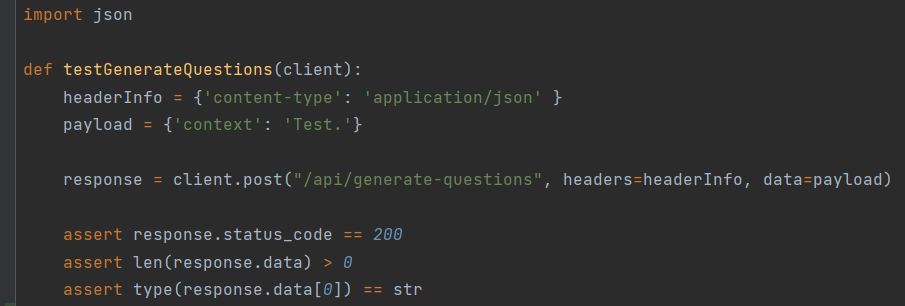
\includegraphics[scale=0.6]{images/test_backend_1.png}
\caption{A szerveroldali végpont egységtesztje.}
\label{fig:tb1}
\end{figure}

A \textbf{qg\_app\_backend} konténerbe terminállal belépve a \textit{pytest} parancs futtatásával lehet elindítani a szerveroldali teszteket. Ekkor minden \textbf{test} szót tartalmazó fájlt tesztnek érzékel és lefuttat a tesztkörnyezet.

\begin{figure}[h]
\centering
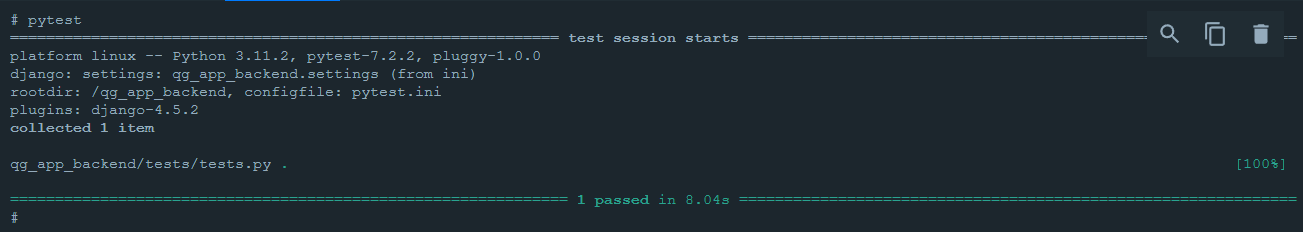
\includegraphics[scale=0.5]{images/test_backend_2.png}
\caption{A szerveroldali tesztek eredménye.}
\label{fig:tb2}
\end{figure}

\pagebreak

Kliens oldalon minden komponenshez készült egységteszt, melyek az adott komponenssel egy mappába kerültek elhelyezésre. Készült továbbá néhány integrációs teszt is az egyes oldalakhoz, illetve az alkalmazás egészéhez.

\begin{figure}[h]
\centering
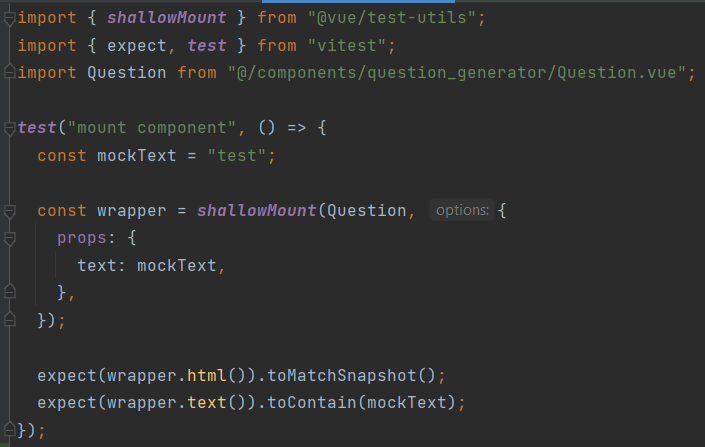
\includegraphics[scale=0.6]{images/test_frontend_1.png}
\caption{Question nevű komponens egységtesztje.}
\label{fig:tf1}
\end{figure}

\begin{figure}[h]
\centering
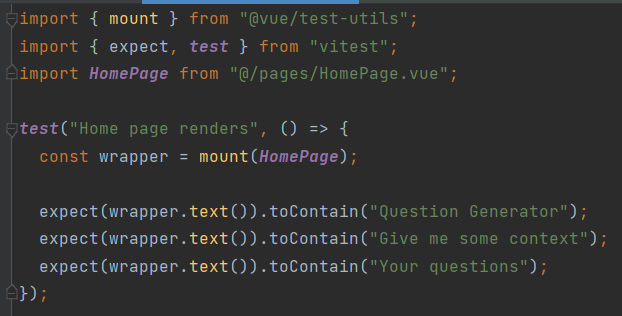
\includegraphics[scale=0.6]{images/test_frontend_2.png}
\caption{A főoldal integrációs tesztje.}
\label{fig:tf2}
\end{figure}

A kliensoldai egységtesztek futtatásához a \textbf{qg\_app\_frontend} konténerbe kell belépnünk és el kell indítanunk a \textit{npm run test} parancsot. Ekkor szintén minden kliensoldali \textbf{test} szót tartalmazó fájlban lefutnak a tesztek.

\pagebreak

\begin{figure}[h]
\centering
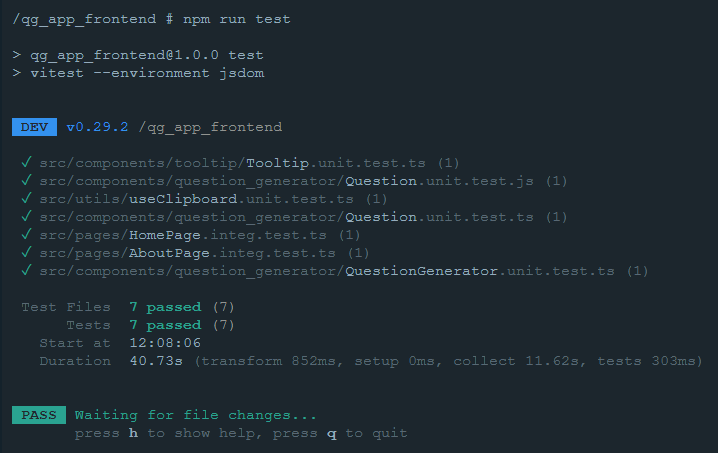
\includegraphics[scale=0.6]{images/test_frontend_3.png}
\caption{A kliensoldali tesztek eredménye.}
\label{fig:tf3}
\end{figure}

\Section{Manuális tesztek}

Mivel alkalmazásunk egy NLP feladat megoldására íródott, így elengedhetetlen, hogy kézzel is teszteljük. Ez esetünkben annyit jelentett, hogy különböző kontextusokat adtunk meg az alkalmazásnak és figyeltük, hogy milyen kérdéseket generált. Egy kérdés akkor számít elfogadottnak, ha értelmes, van köze a kontextushoz és nyelvtanilag is helyes.

A kezdeti tesztek elsősorban az alap működés ellenőrzésére szolgáltak, vagyis hogy képes-e az alkalmazás szavakból, mondatokból vagy hosszabb szövegből kérdéseket generálni.

\begin{itemize}
\item \textbf{Kontextus:} "one"
\item \textbf{Kérdések:} 
	\begin{itemize}
		\item How many questions does one have to answer in order to get a 					good answer?
	\end{itemize}
\item \textbf{Kontextus:} "hungarian"
\item \textbf{Kérdések: }
	\begin{itemize}
		\item What is the nationality of the hungarian population?
		\item What country is the capital of Hungary?
	\end{itemize}
\item \textbf{Kontextus:} "Hungary is a country."
\item \textbf{Kérdések:}
	\begin{itemize}
		\item What is Hungary?
		\item What is a country?
	\end{itemize}
\item \textbf{Kontextus:} "Kate made an apple pie."
\item \textbf{Kérdések:}
	\begin{itemize}
		\item Kate made what kind of pie?
	\end{itemize}
\item \textbf{Kontextus:} "Information technology(IT) is the use of computers to create, process, store, retrieve and exchange all kinds of data and information. IT forms part of information and communications technology(ICT). An information technology system(IT system) is generally an information system, a communications system, or, more specifically speaking, a computer system — including all hardware, software, and peripheral equipment — operated by a limited group of IT users."
\item \textbf{Kérdések:}
	\begin{itemize}
		\item What is the use of computers to create, process, store, retrieve and exchange all kinds of data and information?
		\item IT forms part of what?
		\item What is generally an information system, a communications system, or more specifically speaking a computer system?
	\end{itemize}
\end{itemize}